%% Template para dissertacao/tese na classe ifbathesis
%% versao 1.0
%% (c) 2005 Paulo G. S. Fonseca
%% (c) 2010 Alirío Sá
%% (c) 2012 Antonio Terceiro
%% (c) 2014 Christina von Flach
%% (c) 2016 Alcemir Santos
%% (c) 2018 Luis Gustavo Cardoso Lima
%% https://github.com/gsort/ppgesp-ifba-latex

%% Carrega a classe ifbathesis
%% Opcoes: * Idiomas
%%           pt   - portugues (padrao)
%%           en   - ingles
%%         * Tipo do Texto
%%           bsc  - para monografias de graduacao
%%           msc  - para dissertacoes de mestrado (padrao)
%%           qual - exame de qualificacao de mestrado
%%           prop - exame de qualificacao de doutorado
%%           phd  - para teses de doutorado
%%         * Media
%%           scr  - para versao eletronica (PDF) / consulte o guia do usuario
%%         * Estilo
%%           classic - estilo original a la TAOCP (deprecated) - apesar de deprecated, manter esse.
%%           std     - novo estilo a la CUP (padrao)
%%         * Paginacao
%%           oneside - para impressao em face unica
%%           twoside - para impressao em frente e verso (padrao)

% Atenção: Manter 'classic' na declaracao abaixo:
\documentclass[en, qual, classic, a4paper]{ifbathesis}

%% Preambulo:
\usepackage[utf8]{inputenc}
\usepackage[english]{babel}
\usepackage{graphicx}
\usepackage{lipsum}
\usepackage{hyphenat}
% \usepackage[usenames, dvipsnames, table]{xcolor}
\usepackage{booktabs}
\usepackage{pifont}
\usepackage{multirow}
\usepackage{listings} 
\usepackage{colortbl}
\usepackage{xfrac}
\usepackage[FIGTOPCAP]{subfigure}
\usepackage[printonlyused, withpage]{acronym}
\usepackage{graphicx,url}
%\usepackage[hidelinks,breaklinks]{hyperref}
%\PassOptionsToPackage{hyphens}{url}

\newcommand{\subsubsubsection}[1]{\paragraph{#1}\mbox{}\\}
\setcounter{secnumdepth}{4}
\setcounter{tocdepth}{4}

% Universidade
\university{Instituto Federal da Bahia}

% Endereco (cidade)
\address{Salvador}

% Instituto ou Centro Academico
% nome do departamento ou  área
\institute{Departamento de Pós-Graduação e Qualificação}

% Nome da biblioteca - usado na ficha catalografica
\library{Biblioteca Professor Raul Varella Seixas}

% Programa de pos-graduacao
\program{Programa de P\'{o}s-Gradua\c{c}\~{a}o em Engenharia de Sistemas e Produtos}

% Area de titulacao
\majorfield{Engenharia de Sistemas e Produtos}

% Titulo da dissertacao
\title{A blockchain framework for traceability in supply chain management}

% Data da defesa
% e.g. \date{19 de fevereiro de 2013}
\date{15 de outubro de 2019}
% e.g. \defenseyear{2013}
\defenseyear{2019}

% Autor
% e.g. \author{Jose da Silva}
\author{Edivaldo Mascarenhas Ferreira de Jesus Júnior}

% Orientador(a)
% Opcao: [f] - para orientador do sexo feminino
% e.g. \adviser[f]{Profa. Dra. Maria Santos}
\adviser{Manoel Carvalho Marques Neto}

% Orientador(a)
% Opcao: [f] - para orientador do sexo feminino
% e.g. \coadviser{Prof. Dr. Pedro Pedreira}
% Comente se nao ha co-orientador
\coadviser{Allan Edgard Silva Freitas}

%% Inicio do documento
\begin{document}

\ppgespfrontpage

%% Parte pre-textual
\frontmatter

\ppgesppresentationpage


%%%%%%%%%%%%%%%%%%%%%
% Resumo Portugues e Inglês
%%%%%%%%%%%%%%%%%%%%%
%%%%%%%%%%%%%%%%%%%%%
% Resumo em Portugues
%%%%%%%%%%%%%%%%%%%%%

\resumo
Os avanços nas tecnologias da informação e comunicação reduziram as barreiras físicas, políticas e culturais entre as nações. Essas tecnologias permitiram a globalização ao acesso de matérias-primas, bens e serviços. A complexa rede de relacionamentos que envolve quem fornece materiais, fabricam componentes ou subprodutos, montam ou misturam as partes e entregam o produto final no mercado é conhecida como cadeia de suprimentos. O rápido crescimento das tecnologias da internet permitiu o surgimento de muitas soluções emergentes aplicadas em sistemas de rastreabilidade, na área da cadeia de suprimentos. No entanto, esses sistemas tendem a ser centralizados, monopolistas, assimétricos e opacos. Como conseqüência, essas aplicações resultam em problemas de confiança como fraude, corrupção, adulteração e falsificação de informações. Da mesma forma, por ser um ponto único de falha, o sistema centralizado é vulnerável ao colapso. Atualmente, uma emergente tecnologia chamada blockchain apresenta uma nova abordagem baseada na descentralização. No entanto, por estar em seus estágios iniciais, ela tem alguns desafios a enfrentar, nos quais a escalabilidade e o desempenho se tornam principalmente um desafio para encarar a enorme quantidade de dados no mundo real. Este trabalho pretende fornecer uma estrutura baseada em blockchain para facilitar o desenvolvimento de aplicações para rastreabilidade no gerenciamento da cadeia de suprimentos, usando uma cadeia de recursos minerais como caso de uso.


% Palavras-chave do resumo em Portugues
\begin{keywords}
Blockchain; gerência de cadeia de suprimento; rastreabilidade.
\end{keywords}

%%%%%%%%%%%%%%%%%%%
% Resumo em Ingles
%%%%%%%%%%%%%%%%%%%

\abstract
Advances in information and communication technologies have reduced the physical, political and cultural barriers between nations. These technologies have enabled globalization to access raw materials, goods and services. The complex web of relationships that provide materials manufacture the components, assemble or mix the parts and deliver the final product to market is known as the supply chain. The rapid growth of internet technologies allowed the onset of  lots of emerging technologies applied in traceability systems, in supply chain area. However, these systems tend to be centralized, monopolistic, asymmetric and opaque. As consequence, these systems results in trust problem, such as fraud, corruption, tampering and falsifying information. Likewise, by being a sigle point of failure, centralized system is vulnerable to collapse. Nowadays, a new technology called the blockchain presents a whole new approach based on descentralizatrion. Nonetheless, by being in its early stages, it has some challenges to deal with, in which scalability and performance become  mainly  defiance to face the huge amount of data in the real world. This work is intended to provide a blockchain based framework in order to facilitate the development of applications for traceability in supply chain management using a mineral resource supply chain as use case.

% Palavras-chave do resumo em Ingles
\begin{keywords}
Blockchain; supply chain management; traceability.
\end{keywords}


%%%%%%%%%%%%%%%%%%%
% Sumario / Indice
%%%%%%%%%%%%%%%%%%%

% Comente para ocultar
\tableofcontents

% Lista de figuras
% Comente para ocultar
\listoffigures

% Lista de tabelas
% Comente para ocultar
\listoftables

\chapter*{Lista de Siglas}

% Sintaxe da lista de acordo com a documentação do pacote `acronym'
% documentação: http://mirror.unl.edu/ctan/macros/latex/contrib/acronym/acronym.pdf
\begin{acronym}[PPGESP]
    \acro{PPGESP}{Programa de Pós-Graduação em Engenharia de Sistemas e Produtos}
    \acro{CNPq}{Conselho Nacional de Desenvolvimento Científico e Tecnológico}
    \acro{SCM-BP}{Supply Chain Management - Blockchain Platform}
    \acro{BG}{Byzantine generals}
\end{acronym}

%% Parte textual
\mainmatter

% Eh aconselhavel criar cada capitulo em um arquivo separado, digamos
% "capitulo1.tex", "capitulo2.tex", ... "capituloN.tex" e depois
% inclui-los com:
% \include{capitulo1}
% \include{capitulo2}
% ...
% \include{capituloN}
%
% Importante: 
% Use \xchapter{}{} ao inves de \chapter{}; se n�o quiser colocar texto antes do inicio do capitulo, use \xchapter{texto}{}.

%Seções
\xchapter{Introduction}{}

% É recomendável utilizar `\acresetall' no início de cada capítulo para reiníciar o contator de referências às siglas.
\acresetall 

Hundreds of years ago, supply chains were fairly simple. Mines and farms provided natural resources to skilled craftsman like blacksmiths and Tailors who then created and sold finished products. Today's supply chains are much more complicated, fragmented and difficult to understand. Hundreds or even thousands of supplies all around the world contribute to make and ship products purchased by a customer. Most of the time the various companies don't know about each other and a final consumer likely don't know anything about how, where, when or under what condition the products passed through. This isn't just a problem for consumers. Today's supply chains are so complex that even big industry players have difficulty tracking how their goods get made.

Blockchain and smart contracts could make supply chain management simpler and more transparent. The idea is to create a single source of information about products and supply chain via global ledger. Each component would have its own entry on the blockchain that gets tracked over time. Both untrust companies could then update the status of a good in real-time. The end result is once the clients receive their products they could track every piece back to its manufacturer. Theoretically users could trace the supply chain all the way back to the mines where the raw materials came from \cite{greve2018blockchain}.

Companies can also use the blockchain supply chain as a single source of truth for their products. They can manage and monitor risks within the supply chain, ensure quality of delivery parts and track delivery status of all this. Additionally companies can use smart contracts to manage and pay for supply chain autonomously. For example a chip manufacturer it could be paid immediately upon testing of each individual chip at the assembly facility. This would reduce the need for large contract invoices on the back-and-forth of refund requests for faulty components. Those same smart contracts could assist with shipping and logistics tracking valuable products as they travel around the world. Using blockchain companies can finally have a complete picture of their products at every stage in the supply chain, bringing transparency to the production process while reducing the cost of manufactured goods.

\xchapter{Theoretical Background}{In this section the main concepts studied are presented, which provided subsidies for the development of the proposed project.}


\section{General Context}


\section{Blockchain}
Recently, cryptocurrency has attracted extensive attention from both industry and the academy. Bitcoin, which is often called the first cryptocurrency, had a huge success with the capital market coming to \$ 10 billion in 2016 \cite{coindesk}. Blockchain is the central mechanism of the Bitcoin and was first proposed in 2008 and implemented in 2009 \cite{nakamoto2008bitcoin}. The blockchain can be considered as a public ledger, in which All committed transactions are stored in a block chain. This chain grows continuously when new blocks are attached to it \cite{zheng2016blockchain}.

While the system of financial institutions that serve as third parties reliable processors for processing payments work well for most still suffers from the shortcomings inherent in the model based on confidence. In addition, the cost of mediation increases transaction costs, which limits the practical minimum size of the transaction and eliminates the possibility of small occasional transactions. To solve these problems, \cite{nakamoto2008bitcoin} defined an electronic payment system called Bitcoin, based on cryptographic proof rather than reliable, allowing either party willing to transact directly with each other without the need to a reliable third party.

This revolution began with a new marginal economy on the Internet. Bitcoin emerges as an alternative currency issued and not backed by a central authority, but by automated consensus among networked users. Its true uniqueness, however, lay in the fact that it did not require that users trust each other. Through self-policing algorithmically, any malicious attempt to circumvent the system would be rejected. In a precise and technical definition, Bitcoin is a digital money. which is transacted via the Internet in a decentralized system without bail, using a ledger called blockchain. It's a new way of combining peer-to-peer file sharing rent with public key encryption \cite{swan2015blockchain}.

For \cite{swan2015blockchain}, besides the currency ( "Blockchain 1.0"), smart contracts ("2.0") demonstrate how the blockchain is in a position to become the fifth disruptive computing paradigm after mainframes, PCs, Internet and mobile/ social networks. Bitcoin is starting to become a digital currency, but technology blockchain behind it can be much more significant.

The rapid growth in blockchain technology adoption and the development of applications based on this technology have begun to revolutionize financial services industries. In addition to bitcoin, common applications of blockchain usage varies from proprietary networks used to process financial claims, insurance claims to platforms that can issue and trade equity and corporate bonds \cite{michael2018blockchain}.

Potential benefits of blockchain are more than just economic. They extend to the political, humanitarian, social and scientific domains. Its technological capacity is already being harnessed by specific groups to solve real world problems.

\subsection{Blockchain Properties}\label{sec:propriedades}

Blockchain technology has key features such as centralization, persistence, anonymity and auditability. Blockchain can function in a decentralized environment that is activated by the integration several key technologies such as cryptographic hash, digital signature (based on asymmetric encryption) and distributed consensus engine. With blockchain technology, a transaction may occur in a decentralized manner. As a result, blockchain can greatly save the cost and improve efficiency \cite{zheng2016blockchain}. The main properties of the blockchain are considered innovatively and enable rapid adoption for technology \cite{greve2018blockchain}:

\begin{itemize}
\item Decentralization;
\item Availability and integrity;
\item Transparency and auditability;
\item Immutability and Irrefutability;
\item Privacy and Anonymity;
\item Disintermediation;
\item Cooperation and Incentives.
\end{itemize}
\section{Fundamentals of blockchain}\label{sec:fundamentals}
In this section, the key elements of the blockchain that contribute to its properties will be displayed: integrity, immutability, transparency, availability, disintermediation, decentralization.

\subsection{Cryptography}\label{sec:criptografia}
Blockchain relies heavily on encryption to satisfy system and application security requirements. As the word suggests, cryptocurrencies also make heavy use of encryption. Encryption provides a mechanism for safely encoding the rules of a system encryption on the system itself. This can be used to prevent tampering and misconceptions, as well as coding in a mathematical protocol, the rules for creating new currency units. So, before be able to understand blockchains correctly, it is necessary to understand the cryptographic foundations they trust \cite{narayanan2016bitcoin}.

Cryptography is a deep academic field of research that uses many advanced mathematical techniques that are notoriously subtle and complicated. In this chapter, cryptographic hashes and digital signatures will be defined, which stand out among the most used resources. For more details, the reader should refer to the book \cite{narayanan2016bitcoin}.

\subsubsection{Cryptographic Hashes}\label{sec:hashesCriptograficos}
A hash function is a mathematical function with the three properties to be follow \cite{narayanan2016bitcoin}:

\begin{itemize}
\item  Its input can be any string of any length;
\item Produces a fixed size output. For the purpose of making concrete
the discussion in this chapter (eg., 256 digits);
\item It is efficiently computable. Intuitively, this means that for
a given input string, is possible to find out what is the hash function output within a reasonable period of time. Technically, hashing a n-bit string must have a $O(n)$ runtime.
\end{itemize}

These properties define a general hash function. Cryptographic hash functions (or cryptographic summaries) are unidirectional and hardly allow retrieving the original value $x$ from the hash $h$. For a hash function to be cryptographically secure, it must satisfy the following three properties: (1) collision resistance, (2) hiding and (3) puzzle friendliness \cite{greve2018blockchain}.

A collision occurs when two distinct inputs produce the same output. A hash function $H$ is collision resistant when it is impossible to find two values $x$ and $y$ such that $x \neq y$ and $H(x) = H(y)$ \cite{narayanan2016bitcoin}.

The hide property states that, having the hash function output $y = H (x)$, there is no possible way to find out which whas the $x$ input \cite{greve2018blockchain}.

A hash function $H$ is considered puzzle friendliness if for each possible output value of $n$ bits $y$ if $k$ is chosen from a distribution with high min-entropy, then it is impracticable to find $x$ such that $H (k \| x) = y$ in time significantly less than $2^n$ \cite{narayanan2016bitcoin}.

\subsubsection{Digital Signatures}\label{sec:assinaturasDigitais}
A digital signature is supposed to be a digital analog of a handwritten paper signature. Two signature properties are desired which correspond well to the analogy of the handwritten signature: first, only one person can make their own signature, but anyone can verify if it is valid. Secondly, it is desired that the signature must be linked to a specific document, so the signature cannot be used to indicate the agreement or endorsement to a different document \cite{merkle1989certified}. Moreover, it is not possible to forge a signature in such a way as to reuse it in some other context. That is, signatures must be irrefutable.

To implement digital signatures, asymmetric key encryption is used. A secret key (sk) is used for signing the document and a public key (pk) is used to attest the signature's authenticity \cite{greve2018blockchain}.

A digital signature consists of the following three algorithms \cite{narayanan2016bitcoin}:

\begin{itemize}
\item $(sk , pk) := generateKeys(keysize)$ – The $generateKeys()$ method receives a key size $(keysize)$ in the input and return a pair of public $(pk)$ and private $(sk)$ keys.
\item $sig := sign(sk , msg)$ – The method $sign()$ receives a message $msg$ and a secret key $(sk)$ on entry and returns the signature $sig$ f that message under $sk$.
\item $isValid := veri f y(pk , msg , sig)$ – The method $verify$ receives a public key $(pk)$, a message $msg$ and a signature $(sig)$ as input, and returns a boolean value: $isValid = true$ if $sig$ is a signature valid for $msg$ under $pk$; $isValid = false$, otherwise.
\end{itemize}

The following two properties must be maintained:

\begin{itemize}
\item Authenticity: Signatures can be validated: \\ $verify(pk, message, sign(sk, message)) = = true$.
\item Signatures are existentially unfalsifiable: signature cannot be forged.
\end{itemize}

It is noted that generateKeys() and sign() can be random algorithms. In fact, generating keys should be randomized, because it should be generating different keys for different people. On the other hand, verify() will always be deterministic.

\subsection{Consensus}\label{sec:consenso}
The key to blockchain operation is that the network must agree collectively on the ledger's content. Instead of a central entity maintain control over information (such as a bank for example), the data is shared among all. This requires the network to maintain the consensus around the information recorded in the block chain. How this consensus is reached, affects the security and economic parameters of the protocol \cite{kostarev2017review}.

In this context, consensus emerges as a fundamental problem, since it allow distributed participants to coordinate their actions in order to reach common decisions, thereby ensuring the consistency of safety and system progress (liveness) despite the existence of of failures \cite{greve2018blockchain}. More specifically, in the context of blockchain, consensus enables to reach agreement on the next block that will be added to the blockchain.

In blockchain, reaching consensus between untrusted nodes is a transformation of the problem of \ac{BG} \cite{lamport1982byzantine}. In the BG problem, a group of generals who command a portion of the Byzantine army circles the city. The attack would fail if only part of the generals attacked the city. Generals need to communicate to agree on the attack or not. However, there may be traitors in the generals. The traitor could send different decisions to different generals. This is an environment without trust.

Reaching consensus in such an environment is a challenge. This is also a challenge for blockchain, because its network is distributed and there is no central node that ensures that ledgers on distributed nodes be all the same. Nodes do not need to trust other nodes. Thus, some protocols are required to ensure that ledgers on different nodes are consistent \cite{kostarev2017review}. To solve the consensus problem, several algorithms have been proposed and are listed below. For more details on each algorithm is recommended to read the article \cite{mingxiao2017review}.

\begin{itemize}
\item Proof-of-Work;
\item Proof-of-Stake;
\item Delegated Proof-of-Stake;
\item Leased Proof-Of-Stake;
\item Proof of Elapsed Time;
\item Practical Byzantine Fault Tolerance;
\item Simplified Byzantine Fault Tolerance;
\item Delegated Byzantine Fault Tolerance;
\item Directed Acyclic Graphs;
\item Proof-of-Activity;
\item Proof-of-Importance;
\item Proof-of-Capacity;
\item Proof-of-Burn;
\item Proof-of-Weight;
\end{itemize}

A good consensus algorithm means efficiency, security and convenience. Current common consensus algorithms still have many shortcomings. New consensus algorithms are created to solve some blockchain-specific problems \cite{zheng2016blockchain}.

\subsection{Distributed Ledger}\label{sec:livro}
Distributed ledger is a data structure distributed by several nodes or computing devices. Each node replicates and saves a identical ledger copy. Each participating node in the network updates independently \cite{greve2018blockchain}.

The innovative feature of distributed accounting technology is that the ledger is not maintained by any central authority. Updates to The ledger are independently constructed and recorded by each node. The nodes then vote on these updates to ensure that most agree with the conclusion reached, based on some previous consensus algorithm. Once consensus has been reached, the distributed ledger updates itself and the latest agreed version is saved on each separate node \cite{swan2015blockchain}. Thus, the distributed ledger is replicated and immutable. 

\subsubsection{Transactions}\label{sec:transac}
The blockchain is a public digital book that records online transactions. In it, transactions are recorded in a block without the help of third parties, such as a bank or payment processor. The blockchain algorithm automatically graphs and authenticates the transaction, which is immediately visible to all users, minimizing the possibility of fraud. The terms of transaction do not include any personal or identifying information \cite{Bankrate2018}.

From a technical standpoint, the most fundamental definition of a transaction is an atomic event allowed by the underlying protocol. A transaction determines a sequence of state operations. It adds a transfer of asset or, generally speaking, a smart contract. In a basic case, the transaction girds a digital signature of the issuer holding the asset and the receiver's address, as well as inputs and outputs for transaction. Each transaction must contain both Inputs and Outputs just like in a accounting book. Entries indicate the previous transaction hash which is related to the current one \cite{greve2018blockchain}. Validating a Transition involves:

\begin{enumerate}
	\item signature verification;
	\item confirmation of existing values from hashes of previous referenced transactions;
	\item confirmation that the amount was not previously spent by any other transactions.
\end{enumerate}

In this case, it is necessary to search the blockchain between the block from the referenced transaction to the last block of the structure. Transactions are independently validated by each node of the blockchain network, and this feature contributes to the decentralization of the process \cite{greve2018blockchain}.

\subsubsection{blocks}\label{sec:blocks}
Blocks contains a header with information needed for current maintenance and its validation. A block consists of the block header and block body as shown in Figure \ref{fig:block}. 

\begin{figure}[htbp]
\begin{center}
  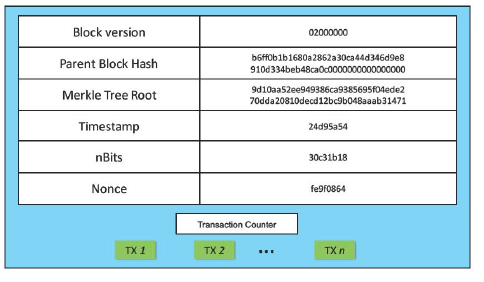
\includegraphics[scale=0.5]{images/blockStructure.png}
\caption{Structure of a block. \cite{zheng2016blockchain}}
\label{fig:block}
\end{center}
\end{figure}

In particular, the header Pack includes:

\begin{itemize}
\item Block version: indicates which set of block validation rules to follow..
\item Parent block hash: A 256-bit hash value that points to the previous block.
\item Merkle tree root hash: The hash value of all transactions in the block.
\item Timestamp: Current date and time as seconds since 1970-01-01T00:00 UTC.
\item  nBits: current hashing target in a compact format.
\item Nonce: A 4-byte field, usually starting with 0 and increasing for each hash.
\end{itemize}

The body's block consists of a transaction counter and transaction. The maximum number of transactions a block can hold depends on block size and the size of each transaction. Blockchain uses a asymmetric encryption mechanism to validate transaction authentication. A digital signature based on asymmetric encryption is used in an untrusted environment \cite{zheng2016blockchain}.

The validation of a block consists in verifying (i) if its structure is well formed (ii) its hash is valid (meets the challenge), (iii) its size is within the network accepted limit, (iv) the set of transactions within the block is valid, (v) the first transaction (and only the first) is the coinbase transaction - which incorporates the generation of new cryptocurrencies in the system, besides acting as a reward mechanism. The blocks are validated independently, by each node of the blockchain network, and this feature contributes to the process decentralization \cite{greve2018blockchain}.

The figure \ref{fig:blockchain} presents a visual representation of a blockchain.

\begin{figure}[htbp]
\begin{center}
  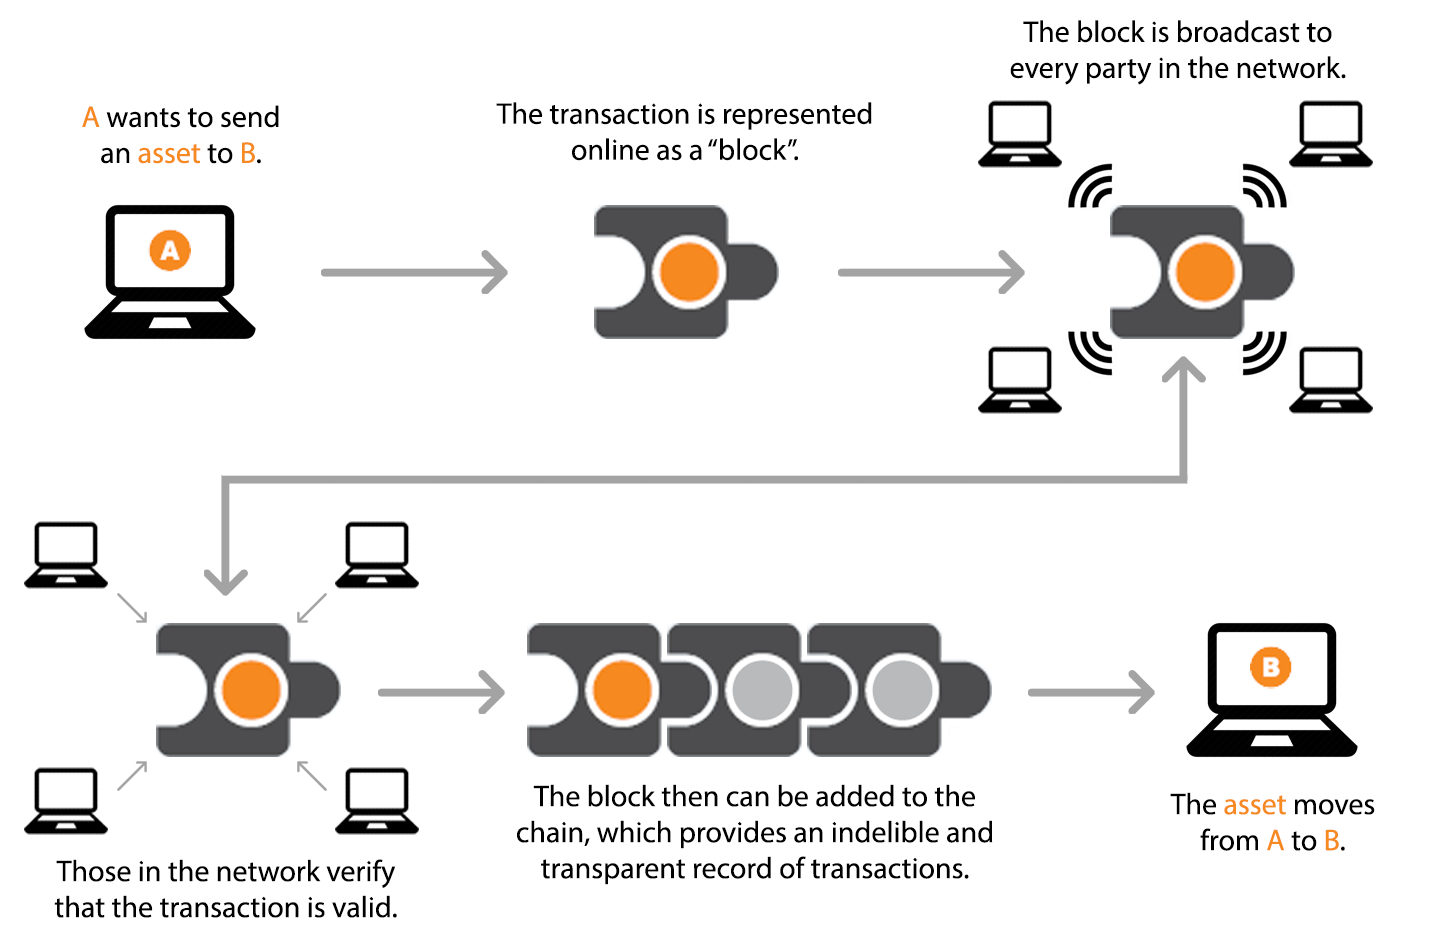
\includegraphics[scale=0.35]{images/blockchain.png}
\caption{Blockchain representation \cite{michael2018blockchain}}
\label{fig:blockchain}
\end{center}
\end{figure}

{\color{red} PAREI aqui. Public Blockchain Versus Private Blockchain}

%MINE
%
text
\xchapter{Technical Specification}{} %sem preambulo

\acresetall 

\ac{SCM-BP} has the general objective to create a generic framework intended to be used in any kind of supply chain correlated to assets and products. 
Craton-Roche SCM-BP is a use case of this framework applied, initially, to the mining supply chain and more specifically, to the gravel ecosystem.

The project will be subdivided into the following specific objectives:
\begin{itemize}
\item Perform a survey of functional requirements.
\item Design system architecture.
\item Develop web application.
\item Develop smart contract.
\item Perform system validations.
\end{itemize}


\section{Application Architecture}\label{sec:applicationArchitecture}

\ac{SCM-BP} is divided into three main modules described below: WebApp - FrondEnd, WebApp - BackEnd and Data Storage. Figure~\ref{fig:detalhamentotecnico} shows the aplication architecture and its components. Figure~\ref{fig:dataStructure} present the main data structure.

\begin{figure}[htbp]
\begin{center}
  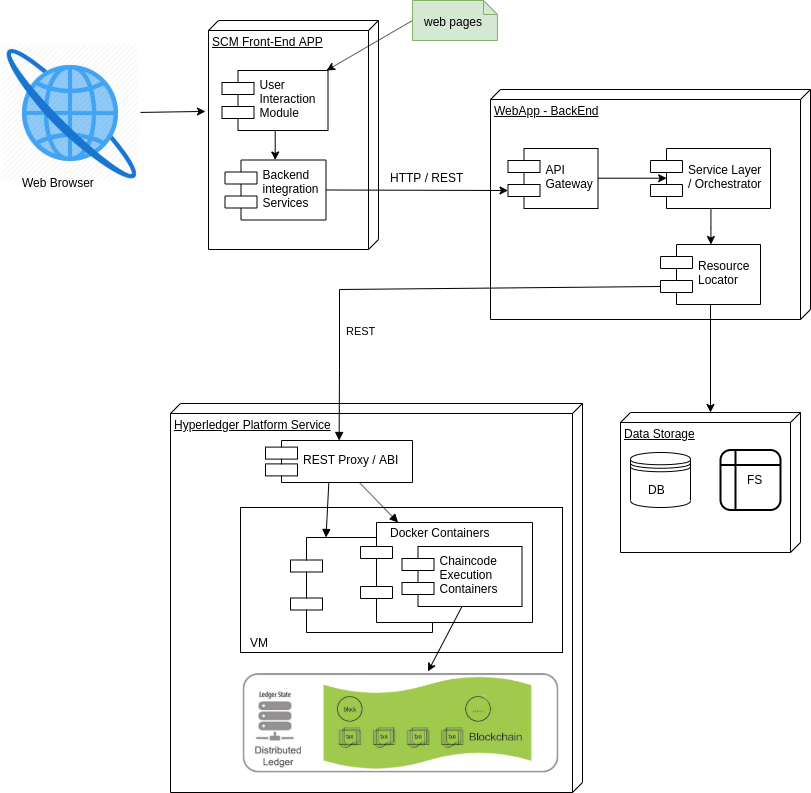
\includegraphics[scale=0.55]{images/detalhamentotecnico.png}
\caption{Application architecture of \ac{SCM-BP}}
\label{fig:detalhamentotecnico}
\end{center}
\end{figure}

\subsection{WebApp - FrondEnd}\label{sec:WebAppFrondEnd}
WebApp - FrontEnd is a client–server computer application which the client (including the user interface and client-side logic) runs in a web browser. This is a single-page application (SPA), a web application that interacts with the user by dynamically rewriting the current page rather than loading entire new pages from a server. This approach avoids interruption of the user experience between successive pages, making the application behave more like a desktop application.

The Application is build with React (also known as React.js or ReactJS). This is a JavaScript library for building user interfaces. It is maintained by Facebook and a community of individual developers and companies. Used as a base in the development of single-page or mobile applications, React is optimal for fetching rapidly changing data that needs to be recorded. However, fetching data is only the beginning of what happens on a web page, which is why complex React applications usually require the use of additional libraries for state management, routing, and interaction with an API.

The Webapp - FrontEnd is divided into two main blocks and these are classified according to the interactions: User Interaction Modules and Backend Interactions Services.

\subsubsection{User Interaction}\label{sec:UserInteraction}
The User Interaction modules are responsible for providing web pages that will be rendered on client’s web browser. These interactions are provided by web pages grouped by the following modules:

\begin{itemize}
\item Login page
\item Application configuration module
\item User handling module (actors - CRUD)
\item Data entry module (forms)
\item Data visualization module
\item Reporting module
\end{itemize}

\subsubsubsection{Login Module}
The Login Module is responsible for display the login and authentication alternatives pages (‘forgot my password’, ‘reset my password’, etc.).

\subsubsubsection{Application configuration module}
The Application configuration module provides the features of creation/configuration of supply chain items and supply chain flows (steps and subtasks).

\subsubsubsection{User handling module}
This module provides the features for creation/configuration of Actors and Roles. The table below show the fields and values for creating a user:

{\color{red}adicionar tabela de criacao de usuario do technical specification aqui.}

\subsubsubsection{Data entry module}
The Data entry module provides form pages that allow users to enter data in the application, search and move assets from a step to another.

\subsubsubsection{Data visualization module}
The Data visualization module is responsible to display the information about assets in the supply chain flow. 

\subsubsubsection{Reporting Module}
In the Reporting module users can generate reports/files containing information organized in a narrative, graphic, or tabular form, prepared on ad hoc, periodic, recurring, regular, or as required basis. Reports may refer to specific periods, events, occurrences, or subjects, and may be presented in written form or any other format.

\subsubsection{Backend Interaction}\label{sec:BackendInteraction}
Backend interactions happen via a service layer consisting of:

\begin{itemize}
\item Authentication service
\item Application setup service
\item User creation service (actors)
\item Data entry service (forms)
\item Data visualization service
\item Reporting service
\end{itemize}

\subsubsubsection{Authentication Service}
The function of the Authentication Service is to request information from an authenticating party, and validate it against the configured identity repository using the specified authentication module. After successful authentication, the user session is activated and can be validated across all web applications participating in an SSO environment. For example, when a user or application attempts to access a protected resource, credentials are requested by one (or more) authentication modules. Gaining access to the resource requires that the user or application be allowed based on the submitted credentials.

\subsubsubsection{Application setup Service}
Application setup service provides methods to configure and edit  supply chain items and supply chain flows, defining which steps and subtasks will be present in this flow and which information will be present in these steps.

\subsubsubsection{User creation Service}
This service is responsible for the creation of users and roles, to allow them to log in and use the application’s features. Only Administrators are allowed to create new users (see Actions and Actors).

\subsubsubsection{Data entry Service}
Data entry service receives data from UI forms and send them to the backend to be processed and stored.

\subsubsubsection{Data visualization Service}
Data visualization services provides information about the supply chain: Assets, users and transactions, to be used by the data visualization module.

\subsubsubsection{Reporting Service}
Report services generate files (Doc/PDF/XSL, etc...) from a specific period of time with information about the supply chain: Assets, users and transactions.
\subsection{WebApp - BackEnd}\label{sec:WebAppBackEnd}
WebApp - BackEnd is a Middleware that runs on the server. This Middleware (server-side software) facilitates client-server connectivity, forming a middle layer between the app(s) and the network: the server, the database, the operating system, and more. It receives requests from the clients (in this case, the WebApp - FrontEnd), and contains the logic to send the appropriate data back to the applicant, over HTTP and REST.  These are the main conventions that provide structure to the request-response cycle between clients and servers. The pair of an HTTP verb and a URI is called a route and matching them based on a request is called routing.

WebApp - BackEnd is an application build with Node.js, an application platform where developers can write Javascript programs that are compiled, optimized and interpreted by the V8 virtual machine. Node.js can create quick, reliable websites and products in much efficient manner. Node.js backend is great for organisations seeking to rapidly prototype an idea. Developing easy to scale real time applications in other technologies is bit difficult, but JavaScript technologies made it easier.

The WebApp - BackEnd is composed by the API Gateway, Service Layer and Resource Locator more detailed below.

\subsubsection{API Gateway}\label{sec:APIGateway}
API Gateway is a managed service that enables easily create, publish, maintain, monitor and secure REST APIs to act as a "gateway" for applications to access data, business logic, or functionality in the backend services, such as workloads. The API Gateway provides a simple uniform view of external resources to the internals of an application. It manages all tasks involved in receiving and processing API calls, including traffic management, authorization and access control, monitoring and management of API versions.

\begin{figure}[htbp]
\begin{center}
  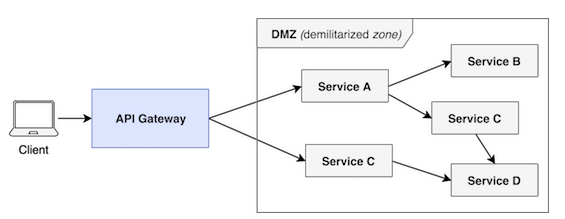
\includegraphics[scale=0.75]{images/apigateway.png}
\caption{API Gateway.}
\label{default-regular2}
\end{center}
\end{figure}

An API is a collection of clearly defined methods of communication between different software components. More specifically, a Web API is the interface created by the back-end: the collection of endpoints and the resources these endpoints expose. A Web API is defined by the types of requests that it can handle, which is determined by the routes that it defines, and the types of responses that the clients can expect to receive after hitting those routes. One Web API can be used to provide data for different front-ends. Since a Web API can provide data without really specifying how the data is viewed, multiple different HTML pages or mobile applications can be created to view the data from the Web API.

Basically, the Gateway is an interface that receives calls to its internal systems, being a large gateway. 

It can act in five different ways:

\begin{itemize}
\item Filter for call traffic from different media (web, mobile, cloud, among others);
\item Single gateway to the various APIs you want to expose;
\item Essential component of API management, as API Suite;
\item Router: API and Rate Limit traffic router;
\item Security engine with authentication, logging and more.
\end{itemize}

Gateway access can be done from many different devices. Therefore, it must have the power to unify outgoing calls and be able to deliver to the user content that can be accessed from any browser and system. The 6 Benefits of a Gateway API:

\begin{enumerate}
\item Application Layer Separation and different requests:
One of the best benefits of this layer is that a gateway can clearly separate implemented APIs and microservices from the people who will actually use them.
\item Increased simplicity for the consumer: Using a Gateway, is possible to show to end user a unique front end with an API collection, and can be much more transparent with API users.
\item Development Improvement: Separation of purposes and functionality not only makes development focus much more on what is really needed, but also helps the server withstand the information demand for the services used. For example, a service that is called a few times a day needs fewer resources than a service called all the time, making the most of the machine's performance.

\item Buffer Zone against attacks: By utilizing multiple standalone Gateway-controlled services, any attack on the application will not affect the overall system, just that service, keeping everything running smoothly. This is the Buffer Zone. In addition to security, this strategy makes it much simpler for the user, as all other features remain normal, not causing stress.

\item Dedication of Services in Favor of User Experience: With the API service independence strategy, a developer can have all the documentation needed to use in a much simpler way, optimizing their time and dedicating themselves exclusively to their activity. This way is possible to usage SDKs for each API separately to make documentation as specific as possible.

\item Activity log anticipating errors: Since all calls to services will go through the Gateway, controlling them all is very simple. This type of log can give the owner of the API a very high power. With it, is possible to find all the errors that can bring down any service, and even who is responsible for a good consumption of the API. This way is easier to predict the number of possible calls avoiding any problems for users.

\end{enumerate}

Gateways as a Security Feature: In the APIs world, one of the most subject talked about issues is always security, and having an API Gateway is one of the best solutions on the market to get full control of API’s, because this pattern addresses the so-called CIA (Confidentiality, Integrity, Availability) almost flawlessly.

\subsubsection{Service Layer}\label{sec:ServiceLayer}
A Service Layer defines an application's boundary [Cockburn PloP] and its set of available operations from the perspective of interfacing client layers. It encapsulates the application's business logic, controlling transactions and coordinating responses in the implementation of its operations.

Enterprise applications typically require different kinds of interfaces to the data they store and the logic they implement: data loaders, user interfaces, integration gateways, and others. Despite their different purposes, these interfaces often need common interactions with the application to access and manipulate its data and invoke its business logic. The interactions may be complex, involving transactions across multiple resources and the coordination of several responses to an action. Encoding the logic of the interactions separately in each interface causes a lot of duplication.

Using service layer pattern provides some benefits:

\begin{enumerate}
\item Centralizes external access to data and functions.
\item Hides (abstracts) internal implementation and changes.
\item Allows for versioning of the services.
\end{enumerate}

The service layer acts as an orchestrator, controlling the flow of incoming and outcoming information requests and responses. Orchestration allows to directly link process logic to service interaction within workflow logic. This combines business process modeling with service-oriented modeling and design, realizing workflow management through a process service model. Orchestration brings the business process into the service layer, positioning it as a master composition controller.

\subsubsection{Resource Locator}\label{sec:ResourceLocator}

Resource locators are components that abstracts the persistence layer. Their job is to provide an object that can help services to discover and persist information from/to the Data Storage Module. Information can be stored in the Blockchain, Filesystem or Database and resource locators should know exactly where get/put data within them.  
\subsection{Data Storage}\label{sec:DataStorage}
Data storage is a general term for archiving data in electromagnetic or other forms for use by a computer or device. Different types of data storage play different roles in a computing environment. In addition to forms of hard data storage, there are now new options for remote data storage, such as cloud computing, and blockchain that can revolutionize the ways that users save and access data.  

Craton-Roche SCM-BP uses three applications as data storages: Blockchain, Cloud filesystem and relational database better detailed on next subsections. 

\subsubsection{Blockchain}\label{sec:DataStorageBlockchain}
A blockchain is a peer-to-peer distributed ledger forged by consensus, combined with a system for “smart contracts” and other assistive technologies. Together these can be used to build a new generation of transactional applications that establishes trust, accountability and transparency at their core, while streamlining business processes and legal constraints.

Craton-Roche SCM-BP uses Blockchain as a supply chain that track parts and service provenance, ensure authenticity of goods, block counterfeits and reduce conflicts.

To achieve that, Hyperledger Fabric is used. Hyperledger is an open source collaborative effort created to advance cross-industry blockchain technologies. It is a global collaboration, hosted by The Linux Foundation, including leaders in finance, banking, Internet of Things, supply chains, manufacturing and Technology.
Hyperledger Fabric is an enterprise-grade permissioned distributed ledger framework for developing solutions and applications. Its modular and versatile design satisfies a broad range of industry use cases. It offers a unique approach to consensus that enables performance at scale while preserving privacy.

In context of Craton-Roche SCM-BP, the Blockchain module consists in a smart contract, chaincode and the ledger. From the application developer’s perspective, a smart contract, together with the ledger, form the heart of a Hyperledger Fabric blockchain system. Whereas a ledger holds facts about the current and historical state of a set of business objects, a smart contract defines the executable logic that generates new facts that are added to the ledger. A chaincode is typically used by administrators to group related smart contracts for deployment, but can also be used for low level system programming of Fabric.

\subsubsubsection{Smart contract}
Before businesses can transact with each other, they must define a common set of contracts covering common terms, data, rules, concept definitions, and processes. Taken together, these contracts lay out the business model that govern all of the interactions between transacting parties.

A smart contract defines the rules between different organizations in executable code. Applications invoke a smart contract to generate transactions that are recorded on the ledger.

\subsubsubsection{Chaincode}
Hyperledger Fabric users often use the terms smart contract and chaincode interchangeably. In general, a smart contract defines the transaction logic that controls the lifecycle of a business object contained in the world state. It is then packaged into a chaincode which is then deployed to a blockchain network. Think of smart contracts as governing transactions, whereas chaincode governs how smart contracts are packaged for deployment.

\subsubsubsection{Ledger}
At the simplest level, a blockchain immutably records transactions which update states in a ledger. A smart contract programmatically accesses two distinct pieces of the ledger – a blockchain, which immutably records the history of all transactions, and a world state that holds a cache of the current value of these states, as it’s the current value of an object that is usually required.

Smart contracts primarily put, get and delete states in the world state, and can also query the immutable blockchain record of transactions.

\begin{itemize}
\item A \textbf{get} typically represents a query to retrieve information about the current state of a business object.
\item A \textbf{put} typically creates a new business object or modifies an existing one in the ledger world state.
\item A \textbf{delete} typically represents the removal of a business object from the current state of the ledger, but not its history.
\end{itemize}

Smart contracts have many APIs available to them. Critically, in all cases, whether transactions create, read, update or delete business objects in the world state, the blockchain contains an immutable record of these changes.

\subsubsection{Filesystem}\label{sec:Filesystem}
A cloud file system is a tiered storage system that provides shared access to file data. Users can create, delete, modify, read and write files, as well as logically organize them into directory trees for intuitive access.

Cloud file sharing can be defined as a service that gives multiple users simultaneous access to a cloud file data set. Cloud file sharing security is managed with user and group permissions, allowing administrators to tightly control access to shared file data.

For all file uploaded and stored in the filesystem, a locally stored digital fingerprint (hash) is saved in the blockchain, separately from the original files or content, to make it easier to confirm whether data has been altered or manipulated in a particular organization.

\subsubsection{Database}\label{sec:Database}
A relational database is a set of formally described tables from which data can be accessed or reassembled in many different ways without having to reorganize the database tables. The standard user and application programming interface (API) of a relational database is the Structured Query Language (SQL). SQL statements are used both for interactive queries for information from a relational database and for gathering data for reports.

\section{Actions And Actors}\label{sec:actionsAndActors}

%%% SETUP

\subsection{Setup}\label{sec:Setup}
Setup is the set of actions to configure the application. Setup phase is when a new supply chain is created or an existing one is updated or deleted. Users can also be created, updated and deleted by setup actions. When creating or editing a supply chain, Admin users will define which steps, substeps and infos the supply chain flow will contain, and which users from member group is allowed to add info and move asset to each step in the logistics network.

\subsubsection{Administrator}\label{sec:Administrator}
Administrator is the only user in Admin group. This actor has access to all areas of the program and have the same abilities that all other user types (configure, move asset and view flow), but his main responsibility is to configure the application, performing the setup actions. 


%%% DATA INSERTION

\subsection{Data Insertion}\label{sec:DataInsertion}

Data insertion are the actions that will fill the supply chain flow with data. Once a new supply chain is created by the admin user, it is ready to be populated with information. Member and admin users are responsible for perform these actions. In Data Insertion phase users can update information from a specific step and substep and move assets depending on the rules applied in the setup phase.

\subsubsection{Raw material/Producer}\label{sec:Rawmaterial}
Providers of raw materials, the quarrier or miner, a gravel producing company. Responsible for the extraction of raw materials (natural resources) and how they are firstly processed (pre-processed) by the suppliers or vendors in order to be delivered to the next stage.

\subsubsection{Manufacturer}\label{sec:Manufacturer}
The same as raw material/producer for gravel, or a machinery/equipment producer. Responsible for the process of converting the raw materials into products that are ready to sell.

\subsubsection{Distributor}\label{sec:Distributor}
Building materials shop or distributor. This actor is responsible of moving the output of the manufacturer (e.g., the product) from manufacturer’s site to a wholesaler and/or retailers.

\subsubsection{Wholesaler}\label{sec:Wholesaler}
Seller of gravel in large quantities, generally to businesses like building companies. Wholesalers in general do not sell products directly to the public, but to other retailers instead.

\subsubsection{Retailer}\label{sec:Retailer}
Seller of gravel in small quantities, generally to natural persons.


%%% VISUALIZATION

\subsection{Visualization}\label{sec:Visualization}

Visualization actions can be performed by any user in the system but its main purpose is to provide to the end user the capability of track the flow off an asset from point of origin to point of consumption.

\subsubsection{End User/ Consumer}\label{sec:EndUser}
The buyer of gravel, either a company or a natural person. Most areas of the program for this user will be unavailable. They will be able only to view the flow of an asset in the supply chain.
%\section{Steps and Substeps}\label{sec:stepsAndSubsteps}

\subsection{Exploration}\label{sec:Exploration}
Exploration is the starting point of a supply chain. Phase which encompasses Mineral Prospecting and Geological Survey.

\subsubsection{Prospecting/ Surveying}\label{sec:Prospecting}
Prospecting means the search of mineral occurrences/surveying means the research on a mineralised area, previously defined during the prospecting phase to be applied as a Mineral Right from the Mining Authority.

\subsubsection{Mining right application}\label{sec:Mining}
Through handing over documents to the Mining Authority (in Brazil it is Agência Nacional de Mineração [ANM]).

\subsubsection{Geological Survey}\label{sec:GeologicalSurvey}
Geological Survey is a set of activities carried out to determine the features on quality and quantity of ore found in a given mineral deposit.

\subsubsection{Mineral reserve definition}\label{sec:MineralReserve}
this step is related to the quantity of ore found during the Geological Survey.

\subsection{Mine Development and Design}\label{sec:MineDevelopment}
In this phase is made the preparation of a deposit to become a mine, opening accesses, setting up fences, building benches.


\subsection{Production}\label{sec:Production}
Production phase including ore extraction and mineral processing or transformation.

\subsubsection{Quarrying/ Blasting plan}\label{sec:Quarrying}
Quantity of stone extracted, same quantity of mineral reserves depleted, type of stone extracted.

\subsubsection{Processing}\label{sec:Processing}
Quantity of stone crushed/processed, same quantity of stone in stock deducted, type of stone product, market requirements.

\subsubsection{Aggregate Product}\label{sec:AggregateProduct}
Listing of products with identified quantities and respective technological features.

\subsection{Distribution}\label{sec:Distribution}
Product distribution with identification of clients and their segmentation. 

\subsubsection{Client by Product Type}\label{sec:Client}
Name, address, size, sector, business registration numbers (federal, state, municipal, county).

\subsubsection{Transport}\label{sec:Transport}
Invoice, bills, type of transportation, weight, distance.

\subsection{Mine Closure}\label{sec:MineClosure}
Mine Closure or mineral decommissioning, it means the end of the mining activity and the start of the installations removal and area remodelling through plantation and/or building a lake.

\subsubsection{Legal Compliance/Decommissioning Plan}\label{sec:LegalCompliance}
Status of all documentation related to the Decommissioning Plan and its Legal Compliance.

\subsubsection{Environmental Recovery/ ANM Application}\label{sec:EnvironmentalRecovery}
Application number and status.

\section{Target Goals}\label{sec:targetGoals}

These are goals for completing specific objectives:

\begin{enumerate}

\item Conduct functional requirements survey. Deadline: 01/06/2019 a 25/06/2019.
\begin{enumerate}
\item Develop application domain understanding;
\item Interact with stakeholders to gather requirements;
\item Classify requirements;
\item Set Requirements Priorities;
\end{enumerate}
\item Design system architecture. Deadline: 26/06/2019 a 25/07/2019.
\begin{enumerate}
\item Define key system modules and components;
\item Establish methods of interaction between components;
\item Make UML Component Diagram;
\item Make use-case UML diagram;
\item Create UML Activity Diagram;
\item Model data structure.
\end{enumerate}
\item Develop Web Application. Deadline: 26/07/2019 a 31/12/2019.
\begin{enumerate}
\item Implement back-end components;
\item Implement front-end components
\end{enumerate}
\item Develop smart contract. Deadline: 05/01/2020 a 29/02/2020.
\begin{enumerate}
\item Implement the chaincode;
\end{enumerate}
\item Perform system validations. Deadline: 01/03/2020 a 30/05/2020.
\begin{enumerate}
\item Perform functional tests;
\item Perform integration tests;
\item Perform security tests;
\item Create acceptance report based on \acf{TAM}.
\end{enumerate}
\end{enumerate}
\section{Scientific Method}\label{sec:method}

For project development, the agile Scrum method has been used. In Scrum, projects are divided into cycles called sprints, with frequent meetings where the team can inform what is being done and think of ways to quickly improve the process. Scrum proposes constant project monitoring. Often the team will be meeting, exchanging experiences, evaluating what has been done and re-planning what will be done next.

During the requirements gathering, developers and other stakeholders sought to raise and prioritize the needs of future software users (referred as requirements). After the requirements gathering, in the requirements specification stage, developers made a detailed study of data collected in the previous activity, from where models were built to represent the software system being developed.

At the architectural design stage of the system two basic activities were performed: architectural design (or high level design), and detailed design (or low level design). Some aspects were considered at this stage of system design, such as: system architecture, platform used, Database Manager System (DBMS) used and graphical interface standard.

In the application development period, the backend and frontend components will be created from the computational description of the design phase. Pre-existing software tools and class libraries will be used to streamline the activity. These tools and libraries will be defined during the architectural design.

For system validation, two main requirements will be evaluated: the components and the behavior of who will use the application. For the first point, functional, integration and security tests will be performed. For the second, the \acf{TAM} method will be used to evaluate user acceptance, utility and ease of use.

The appendix \ref{app:projectManagement} presents the activities for project management, the user stories and non-functional requirements.
%REMOVED
%\xchapter{Exemplos}{} %sem preambulo

A numera\c{c}\~{a}o de figuras \'{e} sequencial, dentro do cap\'{\i}tulo. Ver Figura \ref{default-regular1} e Figura \ref{default-regular2}.

A numera\c{c}\~{a}o de tabelaas \'{e} sequencial, dentro do cap\'{\i}tulo. Ver Tabela \ref{default-table1} e Tabela \ref{default-table2}.


\section{Exemplos de Figura}

\begin{figure}[htbp]
\begin{center}
  
\includegraphics[scale=0.5]{ifba.png}
\caption{Bras\~{a}o do IFBA - Menor.}
\label{default-regular1}
\end{center}
\end{figure}

\begin{figure}[htbp]
\begin{center}
  
\includegraphics[scale=0.75]{ifba.png}
\caption{Bras\~{a}o da IFBA - Maior.}
\label{default-regular2}
\end{center}
\end{figure}

\lipsum

\section{Exemplos de Tabela}
\subsection{Uma Tabela}
\begin{table}[htbp]
\caption{Uma tabela com 3 linhas e 2 colunas.}
\begin{center}
\begin{tabular}{|c|c|} 
\hline
elemento 11 & elemento 12 \\ \hline
elemento 21 & elemento 22 \\ \hline
elemento 31 & elemento 32 \\
\hline
\end{tabular}
\end{center}
\label{default-table1}
\end{table}%

\lipsum

\begin{table}[htbp]
\caption{Uma tabela com 3 linhas e 3 colunas.}
\begin{center}
\begin{tabular}{|l|c|c|} 
\hline
elemento 11 & elemento 12 & elemento 13\\ \hline
elemento 21 & elemento 22 & elemento 23\\ \hline
elemento 31 & elemento 32 & elemento 33\\
\hline
\end{tabular}
\end{center}
\label{default-table2}
\end{table}%

%\xchapter{Outro cap\'{\i}tulo}{} %sem preambulo
\lipsum




%% Parte pos-textual
\backmatter

% Bibliografia
% � aconselh�vel utilizar o BibTeX a partir de um arquivo, digamos "biblio.bib".
% Para ajuda na cria��o do arquivo .bib e utiliza��o do BibTeX, recorra ao
% BibTeXpress em www.cin.ufpe.br/~paguso/bibtexpress
\bibliographystyle{abntex2-alf}
\bibliography{biblio}

% Apendices
% Comente se naoo houver apendices
\appendix

%\lipsum
% Eh aconselhavel criar cada apendice em um arquivo separado, digamos
% "apendice1.tex", "apendice.tex", ... "apendiceM.tex" e depois
% inclui--los com:
% \include{apendice1}
% \include{apendice2}
% ...
% \include{apendiceM}

\xchapter{Data Structure}{} %sem preambulo

{\color{red} Pegar imagem do data structure em casa.}
\begin{figure}[htbp]
\begin{center}
  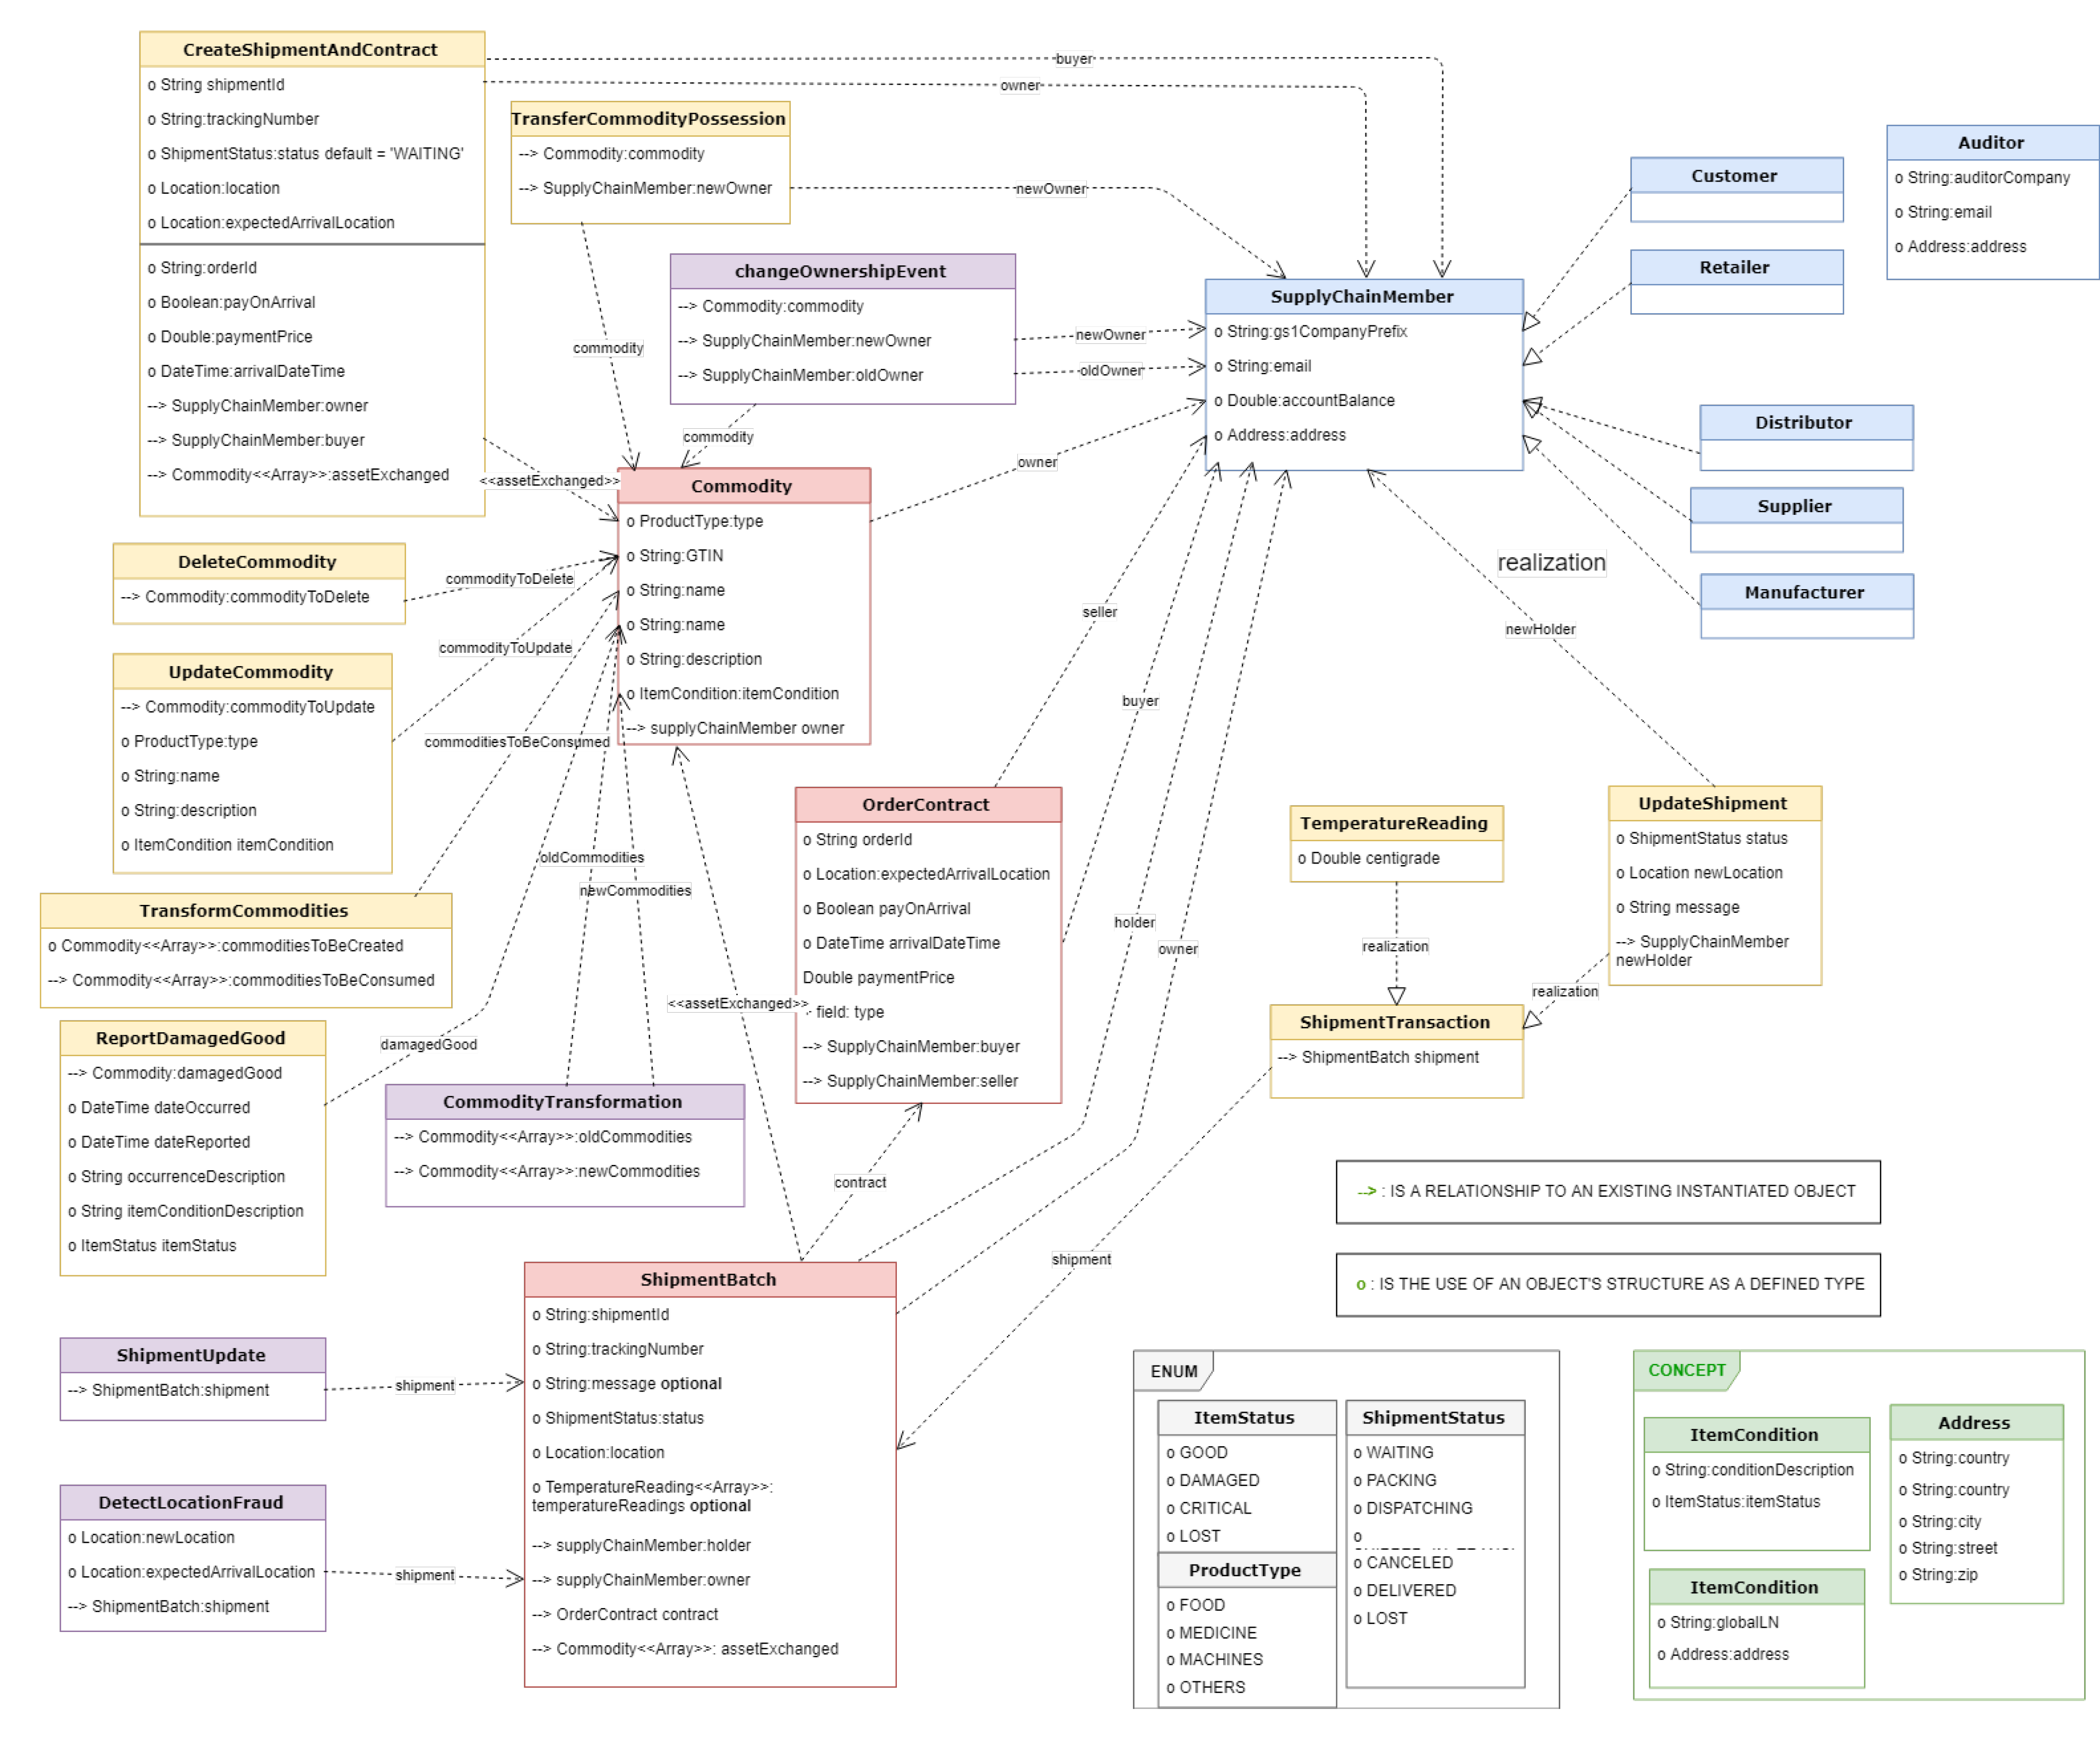
\includegraphics[scale=0.95]{images/classDiagram.png}
\caption{\ac{SCM-BP} data structure}
\label{fig:dataStructure}
\end{center}
\end{figure}
\xchapter{User creation fields}{} %sem preambulo

{\color{red} Adicionar float na tabela abaixo [ht] ??.}
\begin{table}[htpb]
\centering
\caption{User creation service fields}
\begin{tabular}{|p{3cm}|p{12cm}|}
\hline
Field & Input Value \\ 
\hline
User ID & Create a unique identifier for this user's login user name. Duplicated Id is not allowed. \\ 
\hline
First name & Enter the user's full first name. \\ 
\hline
Last name & Enter the user's last name. \\ 
\hline
Title & Enter a title or job description, or select one from the list. \\ 
\hline
Department & Select the user's department from the list. \\ 
\hline
Password & Assign a password to the user. This password can be permanent or temporary. \\ 
\hline
Password needs reset & Select this check box to require the user to change the password during the first login. \\ 
\hline
Locked out & Select this check box to lock the user out of the instance and terminate all their active sessions. \\ 
\hline
Active & Select this check box to make this user active. Only the administrator sees inactive user in: 
\begin{itemize}
\item Lists of users 
\item The selection list on reference fields (magnifying glass icon) 
\item The auto-complete list that appears when you type into a reference field.
\end{itemize} \\ 
\hline
Web service access only & Select this check box to designate this user as a non-interactive user. This field is available with Non-Interactive Sessions. \\ \hline
Internal Integration User & Select this check box to designate this user as an internal integration user. \\ 
\hline
Date format & Select the user's preferred format for dates. \\ 
\hline
Email & Enter the user's email address. \\ 
\hline
Notification & Select the type of notification to send to this user. The default is Email. \\ 
\hline
Time zone & Select the user's time zone. \\ 
\hline
Business phone & Enter this user's business phone number. \\ 
\hline
Mobile phone & Enter this user's mobile phone number. \\ 
\hline
Photo & Attach a photo of the user, if appropriate. \\ 
\hline
Geolocation tracked & Select the check box to enable location tracking. \\ 
\hline
Location & Select the user's usual location. This field is visible when geolocation is active. \\ 
\hline
\end{tabular}
\end{table}
\xchapter{Activities}{} %sem preambulo

Once determined the software architecture and its main modules, these components were divided into activities for better project management. These activities are listed below, segregated by the main modules.

\section{Front end}\label{sec:FrontendActivities}
\begin{itemize}
\item Create login page
\item Create application configuration module
\item Create user creation module (actors)
\item Create data entry module (forms)
\item Create data visualization module
\item Create report module
\item Create authentication service
\item Create application setup service
\item Create user creation service (actors)
\item Create data entry service (forms)
\item Create data visualization service
\item Create reporting service
\end{itemize}

\section{Back end}\label{sec:BackendActivities}
\begin{itemize}
\item Gateway Creation
    \begin{itemize}
    \item Create authentication endpoint
    \item Create application configuration endpoint
    \item Create user creation endpoint (actors)
    \item Create data entry endpoint (forms)
    \item Create data visualization endpoint
    \item Create report endpoint
    \end{itemize}
\item Service Creation
    \begin{itemize}
    \item Create authentication service
    \item Create application setup service
    \item Create user creation service (actors)
    \item Create data entry service (forms)
    \item Create data visualization service
    \item Create reporting service
    \end{itemize}
\item Resource Locator Creation
    \begin{itemize}
    \item Create Connector with Filesystem
    \item Create Connector with Hyperledger Blockchain
    \item Create Connector with Oracle Database
    \end{itemize}
\end{itemize}

\section{Hyperledger Blockchain}\label{sec:HyperledgerBlockchain}
\begin{itemize}
\item Create chaincode (Smart contract)
\end{itemize}

\xchapter{User stories}{} %sem preambulo

The table \ref{table:userStories} present all the user stories for artifacts development, used in the system and managed according to agile methodologies.

{\color{red} Adicionar float na tabela abaixo [ht] ??.}
\begin{table}[htpb]
\caption{\ac{SCM-BP} User Stories}
\label{table:userStories}
    \begin{tabular}{|l|p{13.5cm}|}
    \hline 
    US-1  & As an administrator, clicking “new” on the supply chain list page takes you to the chain configuration page, with empty settings (no phases, subphases, and fields).\\
    \hline 
    US-2  & As an administrator, clicking “edit” on the supply chain list page takes you to the chain configuration page, with the settings filled in (with phases, subphases, and fields already registered). \\
    \hline
    US-3  & As an administrator, when you click delete on the supply chain list page, a modal should appear requesting deletion confirmation.\\
    \hline
    US-4  & As an administrator, when you click confirm deletion on the supply chain list page, an alert should appear stating the deletion result: alert-success or alert-danger.\\
    \hline
    US-5  & As an administrator, on the creation or editing screens of a chain, the administrator must tell from each section which user types can enter information in that section.\\
    \hline
    US-6  & As an administrator, clicking new on the User list page takes you to the user creation page with its empty settings.\\
    \hline
    US-7  & As an administrator, on the user creation page you have to enter the type of user (Admin, Producer, Manufacturer, Distributor, Wholesaler, Retailer, End User).\\
    \hline
    US-8  & As an administrator, clicking “edit” on the User list page takes you to the user creation page, with the settings filled in (with the previously entered data).\\
    \hline
    US-9  & As an administrator, when you click delete on the User list page, a modal should appear asking for deletion confirmation.\\
    \hline
    US-10 & As an administrator, when clicking confirm deletion on the User list page, an alert should appear stating the deletion result: alert-success or alert-danger.\\
    \hline
    US-11 & As "Member" User (Admin, Producer, Manufacturer, Distributor, Wholesaler, Retailer), clicking Move Asset takes you to the information entry page in the chain.\\
    \hline
    US-12 & As "Member", each user can only enter information regarding the allowed phase in the access rules (eg a distributor cannot enter exploration information) as defined in the use case 5.\\
    \hline
    US-13 & As any user (Admin, Member or End User), clicking Track Asset will take you to a page with a list of all assets paged and filtered by date in descending order (most current to oldest).\\
    \hline
    US-14 & As any user (Admin, Member or End User), by clicking on “Track Asset”, the user can enter in the input search an Id to search.\\
    \hline
    US-15 & As any user (Admin, Member or End User), by clicking on “Track”, the user will go to a page with all information of the respective asset, from its conception to the current state.\\
    \hline
    \end{tabular}
\end{table}
\xchapter{Non-functional requirements}{} %sem preambulo

{\color{red} Adicionar float na tabela abaixo [ht] ??.}
\begin{table}[htpb]
\caption{Non-functional requirements of \ac{SCM-BP}}
\label{table:rnf}
\begin{tabular}{|p{3cm}|p{12cm}|}
\hline
NF-1: Usability & The available product, corresponding APIs and documentation should be clear enough to allow for the developers to perform the implementation.\\
\hline
NF-2:  \newline Performance &  \textbf{Speed and latency}:  The throughput and latency on Hyperledger have already been tested, and the throughput is not expected to be as high as in a centralized data system. But, overall, the time to synchronize the information from one company to another might increase; The goal is to make the product be as fast as needed to support the businesses, even if it does not have better performance than other alternatives, since what the target here is the addition of new functionalities (shared ledger); \newline
\textbf{Precision and accuracy}: The product shall record the data just as it was entered, and predictions as to whether a product has any mismatching entries shall always be justifiable; \newline
\textbf{Reliability and availability}: The product shall not always be available unless all of the nodes fail at once, which is almost impossible, unless a coordinated attack were to happen; If some of the nodes happen to fail, the response time of the system might be lower than expected; \newline
\textbf{Scalability}: The product should scale to hundreds of companies, which would require a similar number of nodes;
\\
\hline
NF-3:  \newline Maintainability and portability & The product is expected to run on Linux based systems, compatible with the Docker, nodejs and golang versions that Hyperledger Fabric uses. More specifically, Oracle Cloud services have servers with the required setup for this. Creating new nodes or moving an existing one should be an easy process, without much complication, other than starting the node software on the environment, and closing an existing one, if needed. \\
\hline
NF-4: Security & 
\textbf{Privacy}: The system must ensure appropriate visibility of transactions and products, which might be privacy sensitive; sharing some data would pose a threat or could possibly have negative effects for some of the companies; otherwise, transactions should also be secure, authenticated and verifiable; \newline
\textbf{Immutability}: No one can make changes to the contents of the ledger;\newline
\textbf{Authorization}: All changes to any data should be approved by the people that possess the data or will be affected by these changes directly. A shipment delivery transaction should, for instance, be approved by both the person delivering and the person receiving the shipment. \\
\hline
\end{tabular}
\end{table}



%% Fim do documento
\end{document}
%------------------------------------------------------------------------------------------%
